\documentclass[10pt,a4paper]{article}
\usepackage[T1]{fontenc}
\usepackage[utf8]{inputenc}

\usepackage[margin=2cm]{geometry}
\usepackage{amsmath,amssymb}
\usepackage{longtable,booktabs,array,pdflscape,graphicx}
\usepackage[authoryear,round]{natbib}
\usepackage{xcolor}
\usepackage[hidelinks]{hyperref}
\renewcommand{\thetable}{S\arabic{table}}
\renewcommand{\thefigure}{S\arabic{figure}}
\newcolumntype{P}[1]{>{\raggedright\arraybackslash}p{#1}}
\setlength{\LTcapwidth}{\linewidth}
\begin{document}
\begin{center}
{\Large\bfseries Online Resource 1}\\[4pt]
{\large Supplementary material for ``Quantum Cognition for Robot Decision-Making: A Systematic Review of Quantum-Like Models for Autonomous Agents''}\\[4pt]
Yeshwanth Guru and Dev Kunwar Singh Chauhan\\
Department of Mechanical Engineering, Amrita Vishwa Vidyapeetham, Chennai, India\\
Artificial Intelligence Review
\end{center}

\noindent This resource contains the data-extraction table of the 67 application studies (Table~S1), the PRISMA 2020 checklist (Table~S2), the flow of records (Table~S3 and Figure~S1), the quality-appraisal criteria and judgements (Tables~S4 and S5), the search strategy and the record of the targeted search (Table~S6), the studies excluded under criterion E5 (Table~S7), a glossary of symbols (Table~S8) and the classification of the 71 theory and evidence studies (Table~S9). Section numbers refer to the main article. Tables~S1 and S5 are also provided as CSV files (Online Resources 3 and 4). Evidence levels: E1 conceptual; E2 formal model; E3 human data; E4 simulation or benchmark; E5 physical system; E6 field deployment.


\begin{landscape}
\footnotesize
\begin{longtable}{@{}P{3.0cm}P{2.2cm}P{2.1cm}P{0.6cm}P{4.2cm}P{4.6cm}P{4.4cm}P{1.0cm}@{}}
\caption{Data-extraction table of the application studies ($n = 67$): domain, model type, evidence level, task, key result, main limitation and basis of extraction (full text or abstract). $^\dagger$ also discussed in the companion survey.}\label{tab:S1}\\
\toprule
\textbf{Study} & \textbf{Domain} & \textbf{Model type} & \textbf{Level} & \textbf{Task or phenomenon} & \textbf{Key result} & \textbf{Main limitation} & \textbf{Basis} \\ \midrule
\endfirsthead
\toprule
\textbf{Study} & \textbf{Domain} & \textbf{Model type} & \textbf{Level} & \textbf{Task or phenomenon} & \textbf{Key result} & \textbf{Main limitation} & \textbf{Basis} \\ \midrule
\endhead
\bottomrule
\endfoot

\citet{Moreira2014} & Decision models and networks & Quantum-like & E2 & Probabilistic inference in Bayesian networks under uncertainty & Large departures from classical inference under high uncertainty; collapse to classical under low uncertainty & No human data; free interference phases & Abstract \\
\citet{Moreira2016} & Decision models and networks & Quantum-like & E3 & Sure-thing principle violations (disjunction effect) & Approximates observed violations with automatically set quantum parameters & Heuristic lacks strong psychological justification; aggregate data from few paradigms & Abstract \\
\citet{Moreira2017a} & Decision models and networks & Quantum-like & E3 & Modelling paradoxical human decisions with graphical models & Consolidates quantum-like graphical models reproducing sure-thing violations & Few paradigms; aggregate data; heuristic parameter setting & Abstract \\
\citet{Moreira2020b} & Decision models and networks & Quantum-like & E3 & Decision-making with utilities; paradoxical choices & Predicts observed choice distributions; identifies perceived-optimal but irrational decisions; tracks belief evolution & Interference parameters still required; classic laboratory paradigms only & Abstract \\
\citet{Wichert2020} & Decision models and networks & Quantum-like & E3 & Predicting sure-thing principle violations & Reported accurate prediction of paradoxical decisions without fitted phases & Two paradigms; aggregate data; maximum-entropy assumption & Abstract \\
\citet{She2021} & Decision models and networks & Quantum-like & E4 & Multi-attribute decision making with interacting attributes & Reported better predictive capability than classical Bayesian network approaches & Single application; cognitive interpretation of interference unclear & Abstract \\
\citet{Meghdadi2022} & Decision models and networks & Quantum-like & E3 & Biased human selection in decision games & RMSE 3.4 on Prisoner's Dilemma, ranked first among compared models & Additional loosely constrained parameters; few aggregate datasets & Abstract \\
\citet{Gao2025} & Decision models and networks & Quantum-like & E3 & Sure-thing principle violations; information retrieval & Lowest average and standard deviation of fitting errors among compared models & Existing aggregate datasets; added model complexity & Abstract \\
\citet{Widdows2003} & ML, NLP and IR & Quantum-inspired & E4 & Word-sense disambiguation / retrieval with logical connectives on word vectors & Negation removes unwanted senses (e.g. legal 'suit'); operators equal quantum-logic connectives; no quantitative scores in this paper & Qualitative evaluation only; no human data; non-distributivity not exploited empirically & Abstract \\
\citet{Sordoni2013} & ML, NLP and IR & Quantum-inspired & E4 & Ad hoc document retrieval with term dependencies & Reported competitive or improved retrieval over MRF-style dependency models (numbers not verified here) & Vocabulary-sized density matrices are costly; dependencies are hand-selected; no user/cognitive data & Abstract \\
\citet{Lorenz2023} & ML, NLP and IR & Quantum circuit (QPU) & E5 & Sentence and noun-phrase binary classification (MC, RP) & Hardware test error 16.7\% (MC) and 32.3\% (RP), F-score 0.85/0.75; DisCoCat best on RP & Very small datasets, single hardware run, post-selection overhead, long queue times; no quantum advantage & Full text \\
\citet{Svozil2025} & ML, NLP and IR & Quantum-inspired & E2 & Contextual word embeddings / polysemy & Framework proposal; no quantitative results & No learning procedure, corpus or evaluation; practicality untested & Full text \\
\citet{Stoudenmire2016} & Deep learning and LLMs & Quantum-inspired & E4 & Image classification (supervised learning) & Test-set classification error below 1\% on MNIST & Single simple benchmark; 1-D ordering of 2-D inputs; no cognitive or agent evaluation & Abstract \\
\citet{Zhang2018} & Deep learning and LLMs & Quantum-inspired & E4 & Question answering / answer selection (text matching) & Reported effective against neural and quantum LM baselines (numbers not verified) & Interpretability rests on analogy; text-matching only; no cognitive data & Abstract \\
\citet{Li2019} & Deep learning and LLMs & Quantum-inspired & E4 & Question answering (semantic matching) & Performance comparable to strong CNN and RNN baselines & No gain over baselines; interpretability not user-tested & Abstract \\
\citet{Li2021a} & Deep learning and LLMs & Quantum-inspired & E4 & Multimodal video sentiment analysis (fusion) & Reported competitive with state-of-the-art fusion plus interpretability (numbers not verified) & Task-specific; interpretability argued not measured; no cognitive data & Abstract \\
\citet{Li2021b} & Deep learning and LLMs & Quantum-inspired & E4 & Emotion recognition in conversation (multimodal) & Performance comparable to state of the art & No gain over state of the art; benchmark-only; no human-judgement validation & Abstract \\
\citet{Gkoumas2021} & Deep learning and LLMs & Quantum-like & E4 & Multimodal decision fusion for video sentiment analysis & Substantially outperformed decision- and content-level fusion; handled cases where all unimodal classifiers failed & Incompatibility assumed not tested; benchmark labels, not human decision data & Abstract \\
\citet{Uprety2024} & Deep learning and LLMs & Quantum-like & E4 & Order effects in similarity judgements by LLMs & LLMs show human-like order-effect bias in some settings but not others & Preliminary; prompt-dependent; no QP model fitted in abstract & Abstract \\
\citet{Zhang2025} & Deep learning and LLMs & Quantum-inspired & E4 & Semantic matching / QA & Reported improved/competitive matching (not verified) & Details unverified; density-matrix cost; interpretability not user-tested & Abstract \\
\citet{Maksimovic2025} & Deep learning and LLMs & Quantum-inspired & E4 & Image classification with human-like confidence/uncertainty & Evidence of human-like decision-making; up to 50x faster training than classical counterpart & Human-likeness assessed via simulations, not participant data; datasets unverified & Abstract \\
\citet{Lo2025} & Deep learning and LLMs & Quantum-like & E4 & Contextuality of LLM-derived probabilities in anaphora (co-reference) schema & 77,118 (0.148\%) sheaf-contextual, 36,938,948 (71.1\%) CbD-contextual; Euclidean distance best predictor; rates rise to 0.50\%/81.83\% for similar nouns & Single masked LM; synthetic schema; no downstream-task benefit shown & Full text \\
\citet{Aerts2026} & Deep learning and LLMs & Quantum-like & E4 & Bell-inequality and quantum-statistics tests on LLM concept combination and text & Significant Bell-inequality violation; Bose--Einstein statistics in word distributions, mirroring human data & Prompt/version dependence; signalling not controlled in abstract; interpretive leap to convergent cognition & Abstract \\
\citet{Imannezhad2026} & Deep learning and LLMs & Quantum-like & E4 & Probability judgement fallacies (conjunction, disjunction, complementarity) in GPT-5 vs humans & GPT-5 conjunction fallacies \textasciitilde{}18.8\% vs 58.5\% humans; near-perfect complementarity; pattern closer to early QP models than noisy variants & Single proprietary LLM; personas as proxies; numbers to verify & Abstract \\
\citet{Kang2026} & Deep learning and LLMs & Quantum-like & E4 & Auditing question-order effects in LLM sequential judgements & Near-deterministic saturation in 17/18 and 7/8 pairs; label mapping changed QQ verdicts; no residual contextuality certified & Single small model; few items; saturated measurement interface & Abstract \\
\citet{Dong2008} & Reinforcement learning and agent learning & Quantum-inspired & E4 & Reinforcement learning in unknown environments (gridworld navigation) & QRL learned faster than TD(0) and was robust across a much wider range of learning rates (per preprint) & Only classical simulation of the quantum algorithm; small tabular tasks; claimed parallelism speed-up requires quantum hardware & Abstract \\
\citet{Dong2012}$^\dagger$ & Reinforcement learning and agent learning & Quantum-inspired & E5 & Mobile-robot navigation and obstacle avoidance via RL & QiRL converged in about 2000 episodes across start states (TD 1000--4000); robust for learning rates 0.01--0.12 while TD failed for $\geq$0.02; real robot reached target room after learning & Tabular representation; single TD baseline; real-robot results qualitative & Full text \\
\citet{Briegel2012} & Reinforcement learning and agent learning & Quantum-inspired & E4 & Learning agent design with internal simulation (projective simulation) & Learning curves show a trade-off between forgetting rate and achievable blocking efficiency; larger reflection time speeds learning & Toy environment only; classical simulation; no benchmark comparison with standard RL; quantum version only sketched & Full text \\
\citet{Melnikov2018} & Reinforcement learning and agent learning & Quantum-inspired & E4 & Navigation benchmarks for RL agents (grid world, mountain car) & PS performance similar to Q-learning and SARSA; parameter tuning 1--2 orders of magnitude cheaper & Small tabular tasks; classical only; no deep RL comparison & Abstract \\
\citet{Wei2022} & Reinforcement learning and agent learning & Quantum-inspired & E4 & Experience replay sampling in deep reinforcement learning & Outperforms DRL-PER and DCRL on most games with improved training efficiency (per abstract) & Classical heuristic only; evaluation on game benchmarks; exact gains not verified here & Abstract \\
\citet{Lukac2007} & Robots and embodied agents & Quantum circuit (design or simulation) & E2 & Generating emotional variation in humanoid robot behaviour & Architecture and examples of emotion-modulated behaviour; no quantitative results reported & No evaluation or comparison with classical stochastic models; partial testing; simulated quantum layer & Abstract \\
\citet{Aerts2011d} & Robots and embodied agents & Quantum-like & E1 & Conceptual bridge from quantum cognition to AI and robotics & Proposes a two-layer (classical logical plus quantum conceptual) account of thought and quantum-like structure as a route for AI/robotics & No formal model for robots, no implementation or evaluation; speculative claims about computational power of the mind & Full text \\
\citet{Hangl2016} & Robots and embodied agents & Quantum-inspired & E5 & Hierarchical manipulation skill learning by autonomous play & Robot learned sensing and preparation strategies (e.g., flipping to open box); about 80 roll-outs to reach 90\% success in simulation & Small hand-designed state and skill sets; classical learning; limited task range & Abstract \\
\citet{Yan2019} & Robots and embodied agents & Quantum circuit (design or simulation) & E2 & Representing and transforming robot emotional states & Shows emotion transitions (e.g., anger to relaxation via NOT gates) as unitary operations; argues reduced resource needs & No empirical validation, implementation or classical comparison; benefits require quantum hardware & Abstract \\
\citet{Moreira2020a} & Robots and embodied agents & Quantum-like & E1 & Position on cognitive architectures for decision-making & Proposes quantum-like architecture as a unifying alternative to resource-rational analysis & No formal model specified in detail, no data or implementation; comparative claims not demonstrated & Abstract \\
\citet{Lanza2020} & Robots and embodied agents & Quantum-like & E2 & Robot perception of mutually exclusive percepts & Designed behaviour reproduced in simulation; real quantum hardware showed notable errors & Binary toy scenario; no classical baseline; hardware errors; no demonstrated perceptual benefit & Full text \\
\citet{Hangl2020} & Robots and embodied agents & Quantum-inspired & E5 & Autonomous acquisition of robotic manipulation skills through play & Behaviour composition solved previously unsolvable tasks (e.g., tower disassembly); active learning improved learning speed by about 30\% in simulation & Classical PS only; hand-designed skills; supervision needed; limited scalability evidence & Abstract \\
\citet{Lanza2021} & Robots and embodied agents & Quantum-like & E2 & Multisensory integration and belief representation in robot perception & Measurement probabilities track similarity of inputs to target states; query operators re-map basis meanings consistently & Simulation only; no temporal integration; single query per prepared state; no classical fusion baseline & Full text \\
\citet{Yan2021c} & Robots and embodied agents & Quantum circuit (design or simulation) & E2 & Emotion generation and transition for companion robots & Circuit schemes for generating and transitioning among Plutchik emotions (details not verified) & Apparently formal design only; no verified evaluation or classical comparison & Abstract \\
\citet{Ho2022} & Robots and embodied agents & Quantum circuit (design or simulation) & E2 & Modelling robot affect and user-directed attitude in HRI & Complete circuit framework for affective appraisal, involvement--distance and use intentions & No empirical validation or classical comparison; implementation status unclear & Full text \\
\citet{Song2022} & Robots and embodied agents & Quantum-like & E4 & Pedestrian crossing-intention estimation and trajectory prediction for autonomous vehicles & QLB reported to capture boundedly rational crossings and edge events better than classical probability and Social-LSTM & Narrow scenario; interference parameters not clearly learned; quantitative details not verified here & Abstract \\
\citet{Widdows2023}$^\dagger$ & Robots and embodied agents & Quantum circuit (QPU) & E5 & Implementing quantum cognition models (order effects, disjunction/interference effects) as quantum circuits & Prisoner's Dilemma probabilities (82\%, 73\%, 64\%) reproduced within 0.37\%; order-effect outputs within 2--3\% of expected values & No new human data or fitting; tiny circuits with no quantum advantage; hardware noise affects order-effect circuits & Full text \\
\citet{Mannone2024} & Robots and embodied agents & Quantum circuit (design or simulation) & E2 & Modelling robot 'thinking' and creative behaviour (improvised dance) & Illustrative pose sequences, including feedback-driven unpredictable (creative-like) behaviour and 'overload' responses & Toy model; hand-set states; no behavioural evaluation or classical baseline & Abstract \\
\citet{Daglarli2025}$^\dagger$ & Robots and embodied agents & Quantum circuit (design or simulation) & E4 & Autonomous behaviour of a smart agent (exploration, survival) in a game simulation & Reported 2$\times$ faster convergence to 80\% task success and \textasciitilde{}15\% higher cumulative reward than classical deep RL baseline; gains smaller in reactive, high-uncertainty tasks & Quantum circuits classically simulated; largely qualitative reporting; unclear baselines and statistics; weak justification for algorithm choice & Full text \\
\citet{DeCarolis2025}$^\dagger$ & Robots and embodied agents & Quantum circuit (design or simulation) & E1 & Review and project outline for quantum-enhanced social robotics & Identifies Grover search, quantum walks, PQCs and quantum-inspired emotion models as main tools; recommends hybrid classical--quantum designs given hardware limits & No implementation or evaluation; conflates quantum hardware, quantum-like and quantum-inspired work; limited critical appraisal & Full text \\
\citet{Chella2026} & Robots and embodied agents & Quantum circuit (design or simulation) & E4 & Reactive action selection from robot sensor data (wall following) & Two-sensor configurations best; circuit accuracy about 0.91 (weighted F1 about 0.90); errors near region boundaries & Offline only; no closed-loop robot control; no quantum advantage claimed; hand-defined rule partitions & Abstract \\
\citet{Yukalov2018} & Multi-agent systems and teams & Quantum-like & E2 & Multistep collective decision-making; dynamic disjunction effect & Predicts initial probabilistic deviation, convergence of prospect probabilities to utility factors, and consensus after repeated information exchange; reported to match empirical observations & Stylised interaction rules; validated only against previously published aggregate data & Abstract \\
\citet{Ried2019} & Multi-agent systems and teams & Quantum-inspired & E4 & Collective motion / swarm alignment (marching locusts) & Reproduces density-dependent regimes (disorder, switching alignment, stable alignment); responses converge in \textasciitilde{}10² steps; drift/diffusion qualitatively match experiments & 1-D toy world with two actions; qualitative match only; PS is classical here & Abstract \\
\citet{LopezIncera2020} & Multi-agent systems and teams & Quantum-inspired & E4 & Swarm foraging; emergence of collective motion & Distant food: strong alignment (order parameter $\approx$0.8+), Lévy-like trajectories; near food: weak alignment ($\approx$0.2), Brownian trajectories & 1-D world, two actions, simple reward; PS run classically & Abstract \\
\citet{Lawless2020} & Multi-agent systems and teams & Quantum-like & E1 & Design and control of autonomous human--machine teams & Argues that interdependence behaves quantum-like and that machines in A-HMTs must communicate causally; no quantitative model fit & Conceptual; analogies not formalised or tested quantitatively; case-study interpretation is post hoc & Abstract \\
\citet{Yan2021a}$^\dagger$ & Multi-agent systems and teams & Quantum circuit (design or simulation) & E2 & Representing, transforming and fusing emotional states of social/multi-robot systems & Illustrative probability distributions of fused emotions before and after controlled rotations; qubit count grows logarithmically with robot number but preparation cost is O(2\^{}(4n)) & Conceptual; simulation-only toy examples; no hardware execution, no empirical grounding of emotion model; exponential preparation cost and repeated measurement needed for read-out & Full text \\
\citet{Yukalov2022} & Multi-agent systems and teams & Quantum-like & E2 & Collective decision dynamics in agent networks & Short-memory agents show prolonged probability oscillations; collective information field damps oscillations and forces convergence; reproduces dynamic disjunction effect & Idealised network and communication; no empirical calibration reported in abstract & Abstract \\
\citet{Yukalov2023} & Multi-agent systems and teams & Quantum-like & E2 & Affective (emotion-aware) decision-making for AI & Argues affective AI based on cognition--emotion duality avoids classical behavioural paradoxes & No implementation or empirical test; architecture unspecified & Abstract \\
\citet{Lawless2023}$^\dagger$ & Multi-agent systems and teams & Quantum-like & E1 & Structure and performance of human--machine teams in open systems & Argues team performance is non-decomposable; proposes trade-off between structural and productive entropy production & Mainly review/position; analogical formalism; no new controlled data & Full text \\
\citet{Essalmi2025} & Multi-agent systems and teams & Quantum-inspired & E4 & Interaction-aware decision-making for automated driving (merging, roundabouts) & QG-G4 reported lower collision and higher success rates than baselines; both quantum models give higher expected payoffs than classical games under some parameters & Simulation only; 2$\times$2 games; parameter-dependent; collision results reported as not reproducible by an independent review & Abstract \\
\citet{Kong2026} & Multi-agent systems and teams & Quantum-inspired & E4 & Group navigation and queue formation in swarms & Polarisation $\approx$0.99 within 100 steps; peak elongation ratio 8.31; optimum at moderate granularity (m = 15); polarisation >0.97 under noise up to 30° & Simulation only; PS classical; no physical robots & Abstract \\
\citet{Ashtiani2019} & Human-AI trust & Quantum-like & E4 & Computational trust evolution in multi-agent/decision-support systems & Lower MAE and RMSE than BLADE, TidalTrust, max--min, max--mean and Bayesian methods; malicious recommender amplitude $\approx$0.0009 after 10 iterations & Small synthetic scenarios; no human data; no quantum speed-up & Abstract \\
\citet{Pushparaj2021} & Human-AI trust & Quantum-inspired & E3 & Human--automation trust in air traffic control & Acceptance rate under ambiguous conditions 40\% per participant; model claimed more robust than questionnaire-based models & Very small sample; no reported quantitative model comparison; limited generalisability & Abstract \\
\citet{Humr2023} & Human-AI trust & Quantum-like & E2 & Temporal evolution of human trust in AI-supported decisions & Proposes approach; no quantitative results in abstract & Short proceedings paper; validation not reported in abstract & Abstract \\
\citet{Roeder2023} & Human-AI trust & Quantum-like & E3 & Trust/reliability calibration in human--AI interaction & Quantum model predicted evolving reliability ratings better than Markov model; clear ERP when expectations were perturbed & Exploratory; N = 7; scripted AI behaviour & Abstract \\
\citet{Humr2025}$^\dagger$ & Human-AI trust & Quantum-like & E2 & Human-in-the-loop decision-making with AI support & Illustrative simulations of oscillating confidence; cites \textasciitilde{}15-point question-order effect captured by QP models & No new empirical data; proposals not implemented in an AI system & Full text \\
\citet{vanderMeer2025} & Human-AI trust & Quantum-like & E3 & Dynamics of human trust/reliability ratings in human--AI interaction & Interaction-dependent Hamiltonians reported as a promising means to model trust evolution; no numbers in abstract & Preprint; quantitative evidence not given in abstract; small prior dataset & Full text \\
\citet{Humr2026} & Human-AI trust & Quantum-like & E1 & AI-supported (military) decision-making; human--AI alignment & Three GenAI applications failed to identify conjunction fallacies; QCAL proposed with research agenda & QCAL not implemented or evaluated; GenAI probe small and qualitative & Abstract \\
\citet{Kak2018} & Decision models and networks & Quantum-like & E2 & Order effects in memory and belief queries of intelligent agents & Argues that inaccessible agent states may be best modelled as quantum states; proposes tests on large medical-treatment databases & No data, implementation or quantitative comparison & Abstract \\
\citet{Hoorn2019} & Robots and embodied agents & Quantum circuit (design or simulation) & E2 & Concurrent (mixed) emotions and reflection in robot affect & Circuit examples of robot behaviour under superposed affective states & No simulation results, robot or user study; physical claims about neural quantum dynamics are speculative & Abstract \\
\citet{Essalmi2026}$^\dagger$ & Multi-agent systems and teams & Quantum-inspired & E4 & Interaction-aware decision-making for automated driving with several players & Higher success rates and fewer collisions than classical approaches, especially in highly interactive scenarios & Simulation only; no human drivers or vehicle tests & Abstract \\
\citet{Nebli2026} & Deep learning and LLMs & Quantum-inspired & E2 & Sequence (language) modelling with interference between token paths & Born-rule decoding that keeps phase information is provably more expressive on the constructed task family & No experiments; relevance of interference to natural language untested & Abstract \\
\end{longtable}
\end{landscape}


\begin{longtable}{@{}P{1.2cm}P{4.6cm}P{10.6cm}@{}}
\caption{PRISMA 2020 checklist: location of each item in the main article and this resource.}\label{tab:S2}\\
\toprule \textbf{Item} & \textbf{Topic} & \textbf{Location} \\ \midrule \endfirsthead
\toprule \textbf{Item} & \textbf{Topic} & \textbf{Location} \\ \midrule \endhead
\bottomrule \endfoot

1 & Title & Title page (identified as a systematic review) \\
2 & Abstract & Abstract (unstructured, as required by the journal) \\
3 & Rationale & Sections 1.1--1.4 \\
4 & Objectives & Section 2.1 (RQ1--RQ5) \\
5 & Eligibility criteria & Section 2.3 (I1--I3, E1--E6) \\
6 & Information sources & Section 2.2; Table S6 (sources and dates) \\
7 & Search strategy & Section 2.2; Table S6 (concept blocks of stage 3; exact queries of stage 4) \\
8 & Selection process & Section 2.4 \\
9 & Data collection process & Section 2.5 \\
10a & Data items (outcomes) & Section 2.5; Table S1; Online Resource 3 \\
10b & Data items (other variables) & Sections 2.5 and 2.6 (model type, domain, publication status, basis) \\
11 & Study risk of bias assessment & Section 2.5 (criteria Q1--Q7); Tables S4 and S5 \\
12 & Effect measures & Not applicable: heterogeneous tasks and metrics; no pooled effect (Section 2.6) \\
13a--f & Synthesis methods & Narrative synthesis by domain and evidence level (Sections 2.6 and 14.1); meta-analysis, heterogeneity and sensitivity analyses not applicable \\
14 & Reporting bias assessment & Section 2.6 (threats to validity: publication bias) \\
15 & Certainty assessment & Section 2.6 (evidence levels E1--E6, Table 2) \\
16a & Study selection & Sections 2.2--2.4; Figure S1; Table S3 \\
16b & Excluded studies & Section 2.3; Tables S6 and S7 \\
17 & Study characteristics & Table S1; Online Resource 3 \\
18 & Risk of bias in studies & Section 14.1; Table S5; Online Resource 4 \\
19 & Results of individual studies & Table S1; Sections 7--13 \\
20a--d & Results of syntheses & Sections 5 and 7--13; Section 14.1 and Figure 8 \\
21 & Reporting biases & Section 2.6 \\
22 & Certainty of evidence & Section 14.1; Table 2 \\
23a--d & Discussion & Sections 14--15 and 18; limitations of the review in Section 2.6 \\
24a & Registration & Section 2 (retrospective OSF registration) \\
24b & Protocol & Section 2 (OSF registration) \\
24c & Amendments & Sections 2.2 and 2.3: criterion E5 and the stage 4 search were added after the first corpus was assembled \\
25 & Support & Declarations (no external funding) \\
26 & Competing interests & Declarations \\
27 & Availability of data, code and other materials & Declarations; Online Resources 2--4 \\
\end{longtable}

\begin{longtable}{@{}P{9.5cm}P{6.8cm}@{}}
\caption{Flow of records. Counts for stages 1--3 are works retained after verification; the number of records each search returned and the number excluded at each screening step were not logged and cannot be reported.}\label{tab:S3}\\
\toprule \textbf{Stage} & \textbf{Count} \\ \midrule \endfirsthead
\bottomrule \endfoot
Stage 1: curated reading list, checked against publisher, arXiv or repository records & 102 items listed; about 20 corrected, 3 unlocatable items replaced by 2 verified papers, 2 non-existent titles replaced, 2 dropped \\
Stage 2: authors' PDFs identified by first-page text & 31 works added \\
Stage 3: structured searches and citation chasing (two streams) & 74 works added; records not logged \\
Corpus after stages 1--3 & 205 works \\
Stage 4: targeted search (4 October 2026) and companion-survey cross-check & 17 queries; 10 new records + 1 record; 4 included, 2 excluded, 5 not retrieved (Table S6) \\
Works assessed against I1--I3 and E1--E6 & 209 \\
Excluded as primary studies under E5 (cited once; reviewed in the companion survey) & 11 (Table S7) \\
Application studies (I1), graded & 67 \\
\quad of which appraised against Q1--Q7 (levels E2--E6) & 61 \\
Theory and evidence studies (I2), graded & 71 \\
Reviews and background works (I3), not graded & 17 and 43 \\
Methodological references & 3 \\
Total works cited & 212 \\
\end{longtable}

\begin{figure}[ht]
\centering
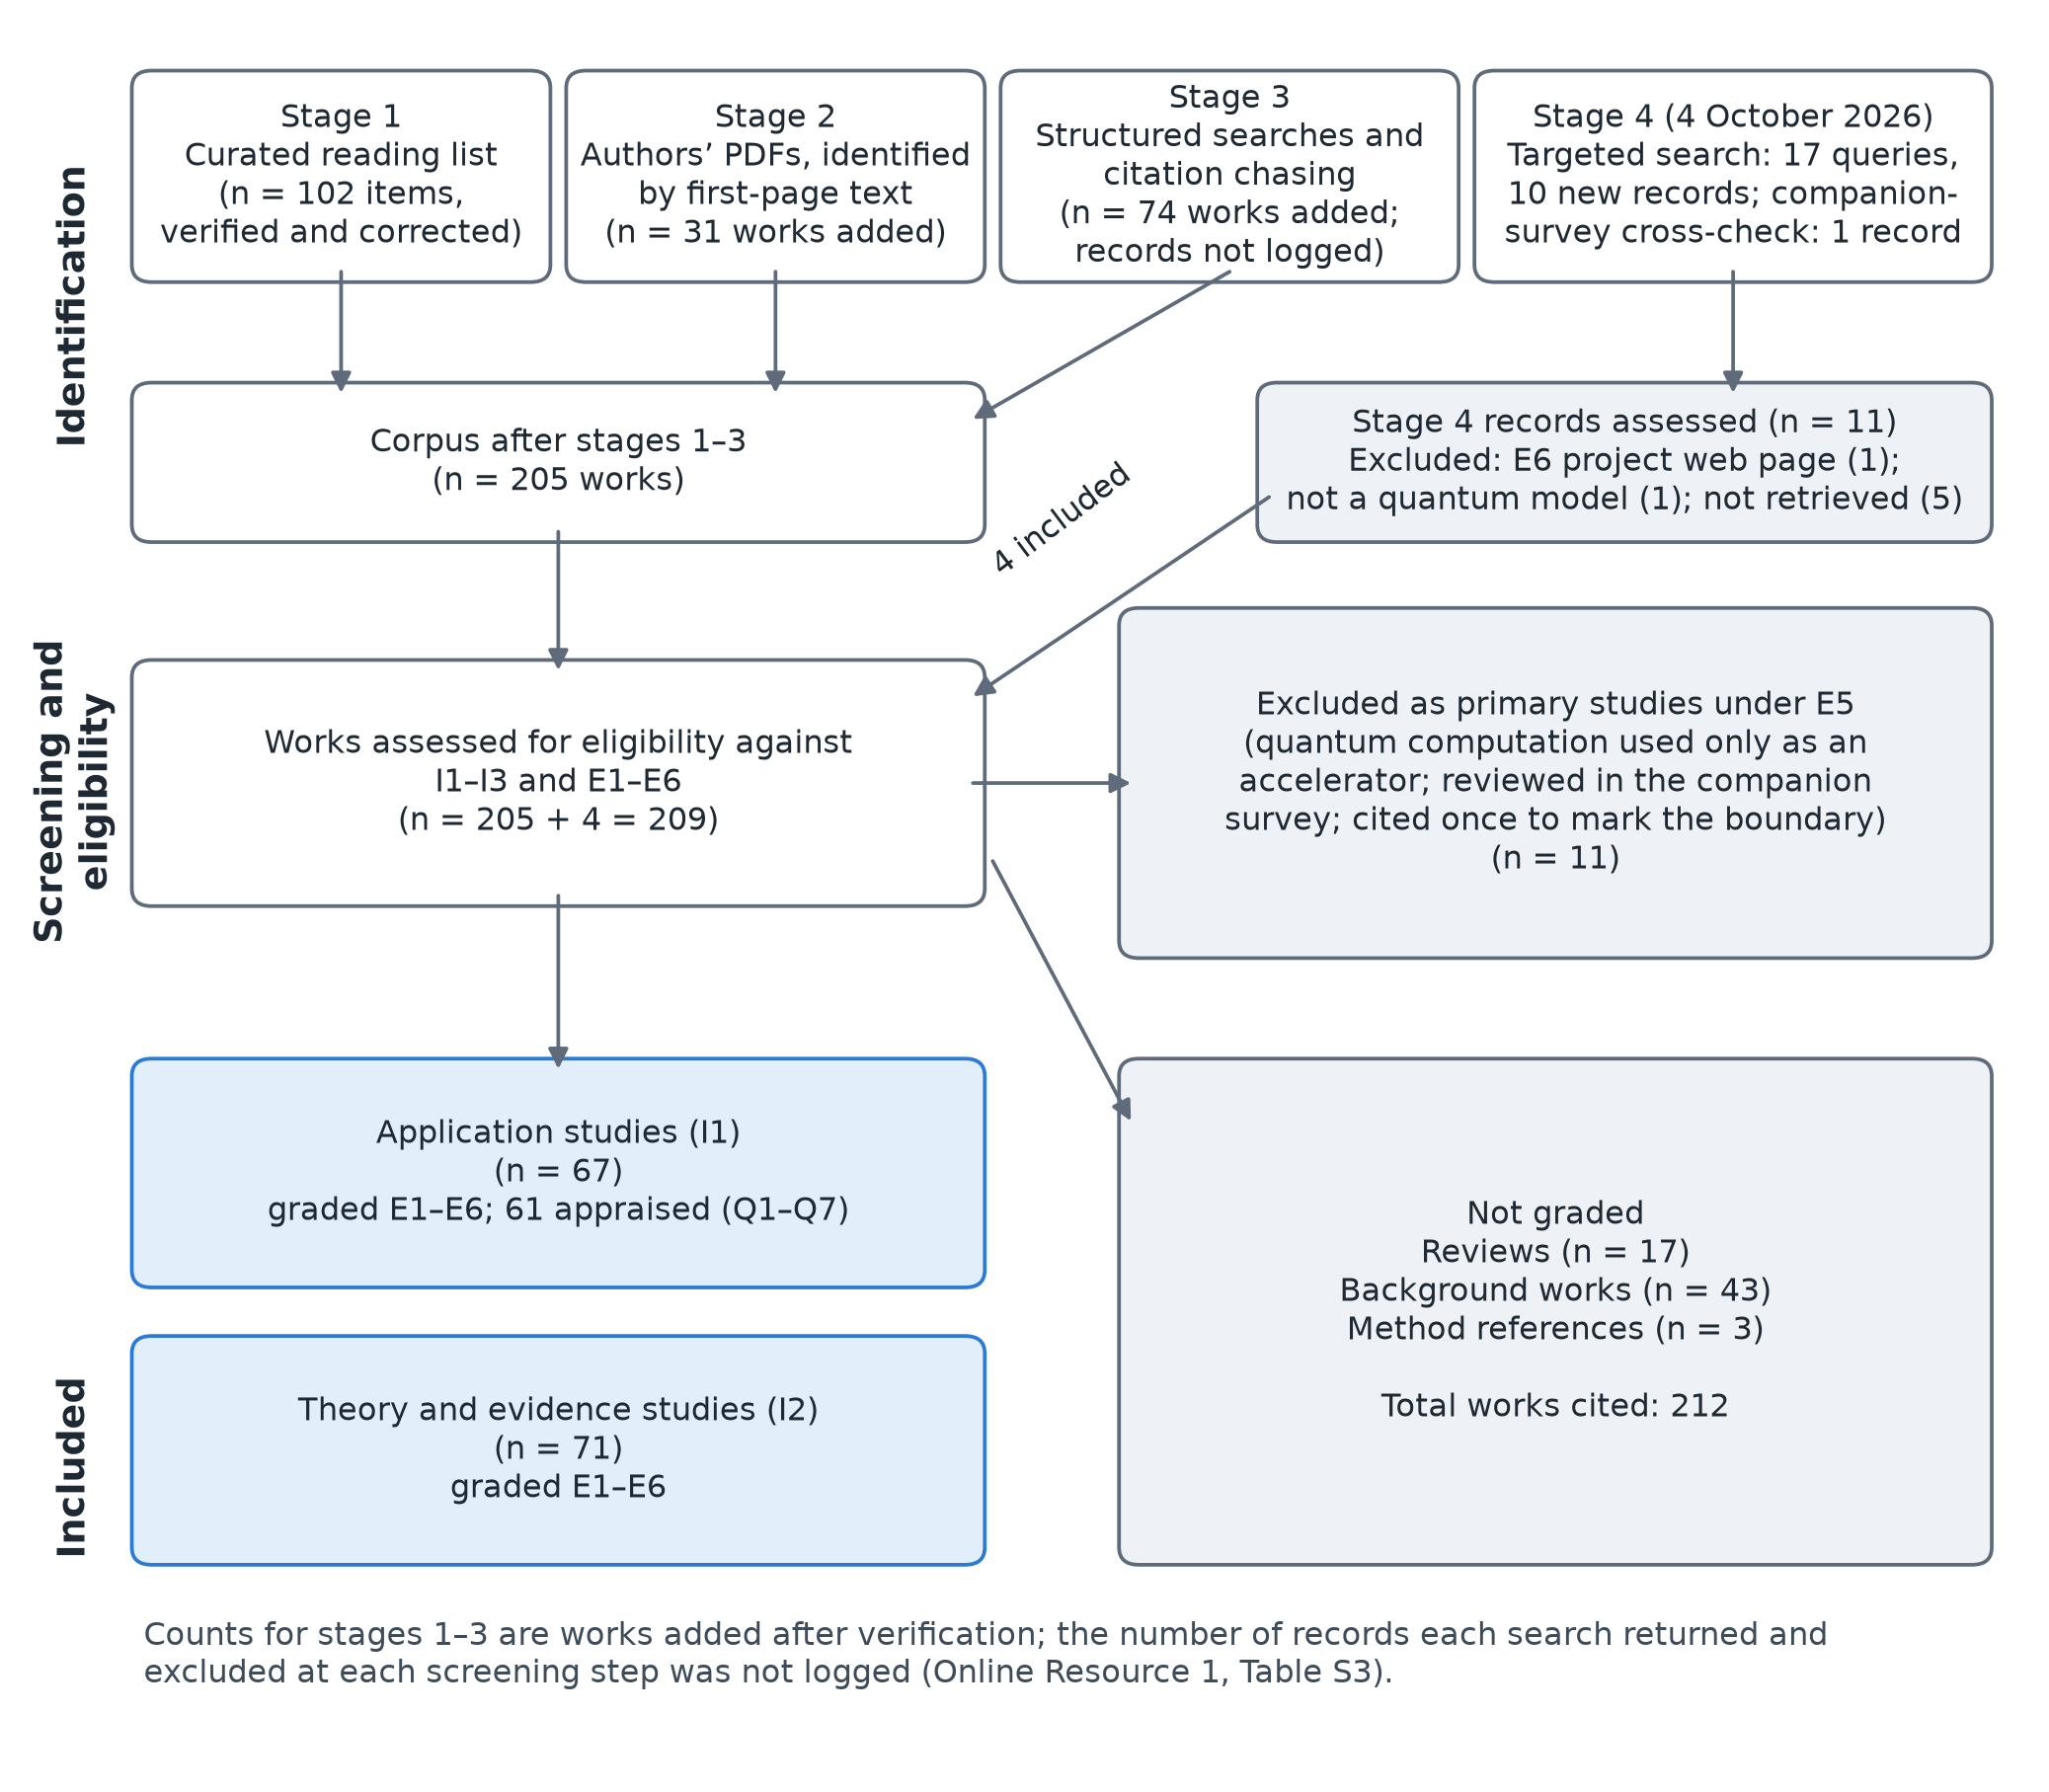
\includegraphics[width=0.92\linewidth]{figures/FigS1_prisma.png}
\caption{Flow of records, following the PRISMA 2020 flow diagram. Stages whose record counts were not logged are marked as such (Table S3).}\label{fig:S1}
\end{figure}


\begin{longtable}{@{}P{0.7cm}P{2.6cm}P{4.6cm}P{4.4cm}P{4.0cm}@{}}
\caption{Quality-appraisal criteria for application studies. Each criterion was judged met (M), partly met (P) or not met (N); the judgements were not summed into a score. Q6 cannot be judged from an abstract and is marked ``?'' when the full text was not available.}\label{tab:S4}\\
\toprule \textbf{ID} & \textbf{Criterion} & \textbf{Met (M)} & \textbf{Partly met (P)} & \textbf{Not met (N)} \\ \midrule \endfirsthead
\bottomrule \endfoot

Q1 & Model specification & State space, state preparation, operators (projectors, instruments, unitaries or Hamiltonians) and free parameters stated. & Model only sketched, or parameters not all stated. & Model not specified. \\
Q2 & Classical comparison & A classical Bayesian, Markov, utility or neural model evaluated on the same task and data. & Classical model discussed but not evaluated on equal terms, or only weak baselines. & No classical comparison. \\
Q3 & Empirical grounding & Human behavioural or neural data, or a realistic agent or AI task. & Narrow benchmark, aggregate data from a few classic paradigms, or a single small case. & Toy example or no data. \\
Q4 & Parameter discipline & Parameters predicted or constrained a priori (e.g., QQ test, phase heuristics), or the model validated on held-out data. & Some parameters constrained, others fitted to the data they explain. & Free parameters fitted to the data they explain, or no evaluation. \\
Q5 & Quantitative evaluation & Metrics reported with variability (repetitions, confidence intervals or tests). & Metrics without variability, or partly qualitative. & Qualitative only. \\
Q6 & Reproducibility & Code and data released. & Code or data released, or the model fully specified in the paper so that it can be re-implemented. & Neither released (``available on request'' counts as not met). \\
Q7 & Critical discussion & Limitations and classical alternative explanations discussed in depth. & Limitations mentioned briefly. & No discussion of limitations. \\
\end{longtable}

\begin{longtable}{@{}P{5.2cm}P{1.6cm}cccccccc@{}}
\caption{Quality appraisal of the 61 application studies at levels E2--E6 (the six conceptual E1 studies are not appraised). M = met; P = partly met; N = not met; ? = not assessable without the full text. Basis: source of the judgements.}\label{tab:S5}\\
\toprule \textbf{Study} & \textbf{Basis} & \textbf{Q1} & \textbf{Q2} & \textbf{Q3} & \textbf{Q4} & \textbf{Q5} & \textbf{Q6} & \textbf{Q7} \\ \midrule \endfirsthead
\toprule \textbf{Study} & \textbf{Basis} & \textbf{Q1} & \textbf{Q2} & \textbf{Q3} & \textbf{Q4} & \textbf{Q5} & \textbf{Q6} & \textbf{Q7} \\ \midrule \endhead
\bottomrule \endfoot

\citet{Moreira2014} & Abstract & M & M & N & N & P & ? & P \\
\citet{Moreira2016} & Abstract & M & P & P & M & P & ? & P \\
\citet{Moreira2017a} & Abstract & M & P & P & P & P & ? & P \\
\citet{Moreira2020b} & Abstract & M & M & P & P & P & ? & P \\
\citet{Wichert2020} & Abstract & M & P & P & M & P & ? & P \\
\citet{She2021} & Abstract & M & M & P & P & P & ? & N \\
\citet{Meghdadi2022} & Abstract & M & M & P & N & M & ? & P \\
\citet{Gao2025} & Abstract & M & M & P & P & M & ? & P \\
\citet{Widdows2003} & Abstract & M & N & P & N & N & ? & P \\
\citet{Sordoni2013} & Abstract & M & M & M & M & M & ? & P \\
\citet{Lorenz2023} & Full text & M & P & P & M & M & M & M \\
\citet{Svozil2025} & Full text & P & N & N & N & N & N & P \\
\citet{Stoudenmire2016} & Abstract & M & P & M & M & M & ? & P \\
\citet{Zhang2018} & Abstract & M & M & M & M & M & ? & P \\
\citet{Li2019} & Abstract & M & M & M & M & M & ? & P \\
\citet{Li2021a} & Abstract & M & M & M & M & M & ? & P \\
\citet{Li2021b} & Abstract & M & M & M & M & M & ? & P \\
\citet{Gkoumas2021} & Abstract & M & M & M & M & M & ? & P \\
\citet{Uprety2024} & Abstract & P & P & M & N & P & ? & P \\
\citet{Zhang2025} & Abstract & P & M & M & M & M & ? & ? \\
\citet{Maksimovic2025} & Abstract & M & M & N & N & P & ? & P \\
\citet{Lo2025} & Full text & M & N & M & M & M & M & M \\
\citet{Aerts2026} & Abstract & P & N & P & M & P & ? & P \\
\citet{Imannezhad2026} & Abstract & M & M & M & M & M & ? & M \\
\citet{Kang2026} & Abstract & M & M & P & M & M & ? & M \\
\citet{Dong2008} & Abstract & M & M & N & P & P & ? & P \\
\citet{Dong2012} & Full text & M & P & M & P & P & N & P \\
\citet{Briegel2012} & Full text & M & N & N & N & P & N & P \\
\citet{Melnikov2018} & Abstract & M & M & P & P & M & ? & P \\
\citet{Wei2022} & Abstract & M & M & M & M & M & ? & P \\
\citet{Lukac2007} & Abstract & P & N & N & N & N & ? & N \\
\citet{Hangl2016} & Abstract & M & P & M & P & M & ? & P \\
\citet{Yan2019} & Abstract & M & N & N & N & N & ? & N \\
\citet{Lanza2020} & Full text & M & N & P & N & P & P & P \\
\citet{Hangl2020} & Abstract & M & P & M & P & M & ? & P \\
\citet{Lanza2021} & Full text & M & N & P & N & P & M & P \\
\citet{Yan2021c} & Abstract & P & N & N & N & N & ? & ? \\
\citet{Ho2022} & Full text & M & P & N & N & N & N & P \\
\citet{Song2022} & Abstract & P & M & M & N & P & ? & P \\
\citet{Widdows2023} & Full text & M & P & P & N & M & P & M \\
\citet{Mannone2024} & Abstract & P & N & N & N & N & ? & P \\
\citet{Daglarli2025} & Full text & P & P & P & N & P & N & N \\
\citet{Chella2026} & Abstract & M & M & P & M & M & ? & M \\
\citet{Yukalov2018} & Abstract & M & P & P & P & P & ? & P \\
\citet{Ried2019} & Abstract & M & P & P & P & P & ? & P \\
\citet{LopezIncera2020} & Abstract & M & N & P & P & M & ? & P \\
\citet{Yan2021a} & Full text & M & N & N & N & P & N & P \\
\citet{Yukalov2022} & Abstract & M & N & N & P & P & ? & P \\
\citet{Yukalov2023} & Abstract & P & N & N & N & N & N & P \\
\citet{Essalmi2025} & Abstract & M & M & P & N & M & ? & P \\
\citet{Kong2026} & Abstract & M & N & P & P & M & ? & P \\
\citet{Ashtiani2019} & Abstract & M & M & P & N & M & ? & P \\
\citet{Pushparaj2021} & Abstract & P & N & M & N & P & ? & P \\
\citet{Humr2023} & Abstract & P & N & N & N & N & ? & P \\
\citet{Roeder2023} & Abstract & M & M & M & P & M & ? & P \\
\citet{Humr2025} & Full text & M & P & N & N & P & N & P \\
\citet{vanderMeer2025} & Full text & M & N & M & P & M & N & P \\
\citet{Kak2018} & Abstract & P & P & N & N & N & ? & P \\
\citet{Hoorn2019} & Abstract & P & N & N & N & N & ? & P \\
\citet{Essalmi2026} & Abstract & M & M & P & N & M & ? & P \\
\citet{Nebli2026} & Abstract & M & N & N & M & N & ? & M \\
\end{longtable}
\noindent Totals (met / partly met / not met / not assessable): Q1 47/14/0/0; Q2 24/16/21/0; Q3 19/24/18/0; Q4 18/16/27/0; Q5 27/22/12/0; Q6 3/2/9/47; Q7 7/48/4/2.

\subsection*{Search strategy}
\noindent\textbf{Stages 1--3.} Sources: Google Scholar, Semantic Scholar, arXiv, PubMed and publisher sites, with backward and forward citation chasing from the main reviews \citep{Pothos2022,Huang2025b,Widdows2021,Meyer2022}. The two search streams covered (a) applications of quantum cognition to robots, agents, human--machine teams and reinforcement learning, and (b) quantum-cognition theory, critiques, machine learning, large language models and neuroscience published from 2016 to 2026. The exact strings and record counts were not logged. To support replication, the following concept blocks reproduce the scope of the two streams; they are a reconstruction, not a log:

\begin{quote}\small
(\texttt{"quantum cognition" OR "quantum-like" OR "quantum probability" OR "quantum decision theory" OR "quantum-inspired" OR "projective simulation"})\\
AND (\texttt{robot* OR agent* OR "human-robot" OR autonomous OR "multi-agent" OR swarm OR "reinforcement learning" OR "machine learning" OR "language model*" OR trust OR automation})\\
\emph{or}, for stream (b), AND (\texttt{"order effect*" OR "conjunction fallacy" OR "disjunction effect" OR "sure-thing" OR interference OR contextuality OR "Bayesian network*" OR critique})
\end{quote}

\noindent\textbf{Stage 4 (4 October 2026).} Exact queries, results and decisions are given in Table~S6.


\begin{longtable}{@{}P{1.3cm}P{7.6cm}P{7.4cm}@{}}
\caption{Targeted search of 4 October 2026: queries and decisions. The full log, including the verification queries, is in the method workbook (targeted\_search\_record.md).}\label{tab:S6}\\
\toprule \textbf{\#} & \textbf{Query} & \textbf{New records and decisions} \\ \midrule \endfirsthead
\bottomrule \endfoot

T1 & \texttt{quantum-like model human-robot interaction decision-making robot 2024 2025} & Genoa research-project page (excluded, E6) \\
T2 & \texttt{quantum cognition large language model order effects 2025 arXiv quantum probability} & Kak (2018) and Nebli et al. (2026) (included); arXiv:2510.13894 (not retrieved) \\
T3 & \texttt{quantum probability model trust automation human-autonomy teaming 2024 2025 study} & Flight-test trust case study (excluded, not a quantum model); arXiv:2410.20496 and arXiv:2503.16227 (not retrieved) \\
T4 & \texttt{quantum-like Bayesian network decision support autonomous driving or robot 2023 2024 2025} & No new record \\
T5 & \texttt{quantum decision theory artificial agents reinforcement learning quantum-like agent Yukalov 2024 2025} & No new record \\
T6 & \texttt{quantum-inspired cognitive model robot emotion social robot 2024 2025 quantum-like} & Hoorn and Ho (2019) (included); J. Phys.: Conf. Ser. 2115, 012040 (not retrieved) \\
V1--V11 & Eleven verification queries (titles, authors and abstracts of the records above) & arXiv:2608.14691 seen as a title only (not retrieved) \\
Other & Cross-check against the companion survey's corpus & Essalmi et al. (2026) (included) \\
\end{longtable}

\begin{longtable}{@{}P{4.6cm}P{11.7cm}@{}}
\caption{Studies excluded as primary studies under criterion E5 (quantum computation used only to accelerate a robot or learning task, without a cognitive or decision model). They are reviewed in the companion survey \citep{Guru2026} and cited once in the main article to mark the boundary.}\label{tab:S7}\\
\toprule \textbf{Study} & \textbf{Method} \\ \midrule \endfirsthead
\bottomrule \endfoot

\citet{Chen2020} & Variational quantum circuits as Q-function approximators \\
\citet{Jerbi2021} & Parametrised quantum policies; learning separations on constructed tasks \\
\citet{Skolik2022} & Variational deep Q-learning (CartPole) \\
\citet{Acuto2022} & Variational quantum soft actor-critic for a simulated arm \\
\citet{Sinha2023} & Quantum critic for self-driving navigation (Nav-Q) \\
\citet{Hohenfeld2024} & Variational deep Q-learning for robot navigation \\
\citet{Yun2022} & Quantum multi-agent reinforcement learning \\
\citet{Paparo2014} & Quantum speed-up of agent deliberation (quantum walks) \\
\citet{Chella2022} & Grover search for robot motion planning \\
\citet{Mannone2022} & Quantum-circuit models of swarm interaction rules \\
\citet{Khoshnoud2020} & Quantum communication for cooperating robots \\
\end{longtable}

\begin{longtable}{@{}P{4.2cm}P{12.1cm}@{}}
\caption{Glossary of symbols and notation.}\label{tab:S8}\\
\toprule \textbf{Symbol} & \textbf{Meaning} \\ \midrule \endfirsthead
\bottomrule \endfoot

$|\psi\rangle$, $\langle\psi|$ & State vector (ket) and its conjugate transpose (bra) \\
$\langle\phi|\psi\rangle$ & Inner product \\
$\rho$ & Density matrix (mixed state); $\mathrm{tr}\,\rho = 1$, $\rho \succeq 0$ \\
$P_A$ & Projector onto the ``yes'' subspace of question A \\
$I - P_A$ & Projector onto the ``no'' subspace \\
$[A, B] = AB - BA$ & Commutator; zero for compatible questions \\
$\lVert P|\psi\rangle\rVert^2$ & Born-rule probability \\
$U(t) = \exp(-iHt)$ & Unitary evolution generated by Hamiltonian $H$ \\
$L_k$, $\gamma_k$ & Lindblad (jump) operators and rates in open-system models \\
$\otimes$ & Tensor product of spaces or states \\
$\theta$ & Interference phase between two branches \\
QQ & Quantum question equality \\
QLBN & Quantum-like Bayesian network \\
QRL, QiRL & Quantum and quantum-inspired reinforcement learning \\
PQC, VQC & Parametrised and variational quantum circuit \\
PS & Projective simulation \\
CbD & Contextuality-by-default \\
POVM & Positive-operator-valued measure (generalised measurement) \\
QPU & Quantum processing unit \\
\end{longtable}

\footnotesize
\begin{longtable}{@{}P{3.6cm}P{0.7cm}P{4.6cm}P{6.2cm}P{1.1cm}@{}}
\caption{Theory and evidence studies ($n = 71$), graded on the evidence scale: phenomenon, key result and basis of extraction.}\label{tab:S9}\\
\toprule \textbf{Study} & \textbf{Level} & \textbf{Phenomenon} & \textbf{Key result} & \textbf{Basis} \\ \midrule \endfirsthead
\toprule \textbf{Study} & \textbf{Level} & \textbf{Phenomenon} & \textbf{Key result} & \textbf{Basis} \\ \midrule \endhead
\bottomrule \endfoot

\citet{Khrennikov1999} & E2 & Formal description of cognitive and social information processes & No empirical results; provides a p-adic formalism for information dynamics & Full text \\
\citet{Aerts2000} & E2 & Logical structure of disjunction; concept combination & Quantum disjunction shown non-equivalent to classical 'or' owing to EPR-like correlations & Abstract \\
\citet{Busemeyer2006} & E2 & Choice and response-time dynamics in decision-making & Quantum dynamics produce interference effects not possible under Markov models; predictions contrasted & Abstract \\
\citet{Pothos2009} & E3 & Sure-thing principle violations in prisoner's dilemma and two-stage gambles & Interference reproduces violations of the law of total probability that classical models cannot & Abstract \\
\citet{Busemeyer2009} & E3 & Choosing between Markov and quantum dynamic models of decision & Provides parameter-free tests discriminating Markov vs quantum models; evidence reviewed on both properties & Abstract \\
\citet{Aerts2009} & E3 & Concept combination; membership weights for conjunctions and disjunctions & Data shown incompatible with classical models; quantum model reproduces over- and underextension & Full text \\
\citet{Khrennikov2010} & E2 & Foundations of quantum-like modelling in psychology, economics and finance & Systematic quantum-like framework linking contextuality and interference to QP representations & Abstract \\
\citet{Trueblood2011} & E3 & Order effects in sequential evidence evaluation (inference) & Quantum model reproduced the pattern of order effects better than the anchoring-and-adjustment model (per Bruza 2015) & Abstract \\
\citet{Busemeyer2011} & E3 & Probability judgement fallacies (conjunction, disjunction, inverse, conditional) & Quantum model explains more of 15 major findings than three rival theories & Full text \\
\citet{Aerts2011a} & E3 & Concept combination; entanglement between concepts & CHSH value 2.4197 > 2, interpreted as violation of Bell's inequality & Full text \\
\citet{Aerts2011b} & E2 & Concept combination, decision paradoxes and information retrieval & Argues quantum structure is a structural model for human and artificial thought; proposes SCoP-based knowledge organisation & Full text \\
\citet{Aerts2011c} & E3 & Sure-thing principle violations; disjunction effect (Hawaii problem) & Quantum model reproduces 54\%/57\% vs 32\% choice pattern as interference of conceptual landscape & Full text \\
\citet{Yukalov2011} & E3 & Decision under risk and uncertainty; classical paradoxes & Explains disjunction effect, conjunction fallacy, Allais and Ellsberg-type paradoxes & Abstract \\
\citet{Busemeyer2012} & E3 & Order effects, judgement errors, concepts, memory, decision dynamics & Unified QP account of multiple anomalies; comparisons with classical/Markov models & Full text \\
\citet{Pothos2013a} & E3 & General case for QP cognitive modelling & Argues many judgement and decision anomalies have natural QP accounts & Full text \\
\citet{Wang2013a} & E1 & Programmatic case for quantum models of cognition & Frames QP as a general cognitive modelling framework and lists open questions & Abstract \\
\citet{Wang2013b} & E3 & Question order effects in attitude surveys & QQ equality supported in the data examined & Abstract \\
\citet{Aerts2013} & E3 & Concept combination and conceptual dynamics & Quantum models reproduce guppy-type effects, over/underextension and entanglement & Abstract \\
\citet{Wang2014} & E3 & Question order effects in national surveys & QQ equality statistically supported; anchoring-adjustment models fail to reproduce patterns & Abstract \\
\citet{Khrennikov2014} & E2 & Consistency of quantum measurement models with order effects and response replicability & Projective quantum models cannot jointly reproduce order effects and response replicability & Abstract \\
\citet{Bruza2015} & E3 & Review of quantum vs Bayesian models of judgement and decision & QP accounts for order effects, QQ equality (70 surveys), total-probability violations; classical and QP coincide for compatible events & Full text \\
\citet{Busemeyer2015} & E1 & Introduction to quantum cognition for psychologists & Summarises QP explanations of order effects, fallacies and sure-thing violations & Abstract \\
\citet{Kvam2015} & E3 & Choice-confidence interference in perceptual evidence accumulation & Intermediate choice changed later confidence (interference); quantum walk fitted better than Markov & Abstract \\
\citet{Yearsley2016a} & E2 & Tutorial on constructing quantum cognitive models & Step-by-step construction of order-effect models and derivation of the QQ equality & Abstract \\
\citet{Wang2016} & E3 & Interference of categorisation on decision-making & Interference (violation of total probability) in some conditions; BAE model predicted the pattern & Abstract \\
\citet{Yearsley2016b} & E3 & Effect of repeated judgements on belief change (quantum Zeno effect) & Frequent judgements associated with slower belief change, consistent with a Zeno effect & Abstract \\
\citet{Yukalov2016} & E2 & Foundations of quantum probability for measurement and decision-making & Predicted 0.35/0.65 vs observed 0.37/0.63 cooperation/defection; conditions for classical reduction & Full text \\
\citet{Dzhafarov2016a} & E2 & Defining and testing contextuality in systems of random variables & Criterion distinguishing true contextuality from direct context influences on marginals & Abstract \\
\citet{Yearsley2017} & E2 & Tutorial on advanced quantum-cognition tools & Framework for incorporating noise and imperfect measurement in QP models & Abstract \\
\citet{Pothos2017} & E2 & Normative (rational) status of quantum probabilistic judgement & Argues QP reasoning can be principled rather than simply erroneous under incompatible perspectives & Abstract \\
\citet{Trueblood2017a} & E3 & Probabilistic inference judgements (order effects, inverse fallacy, Markov violations, anti-discounting) & Accounts for five inference phenomena; representations become more classical with task familiarity & Abstract \\
\citet{Broekaert2017} & E2 & Time evolution of mental states in decision-making & Clarifies relations and explanatory value of increasingly complex dynamics & Abstract \\
\citet{Aerts2017} & E4 & Conjunction fallacy & Emergence effects, not order effects, identified as the main mechanism & Abstract \\
\citet{Aerts2017b} & E3 & Question order effects and response replicability in sequential survey judgements & Exact fits to both data sets; argues the data are irreducibly non-Hilbertian, that the QQ-equality can hold for non-Hilbertian models, and that order effects plus replicability are jointly modelled & Full text \\
\citet{Busemeyer2018} & E3 & Context effects across subsets of judged variables & HSM fits compare favourably with Bayesian networks, demonstrating viability & Abstract \\
\citet{Cervantes2018} & E3 & Contextuality in paired human choices & Marginal selectivity violated, yet true contextuality detected beyond direct influences & Abstract \\
\citet{Busemeyer2019} & E3 & Belief change during evidence monitoring; sequential probability ratings & Small interference effects (low coherence; 3/11 participants); summed G² diff favoured quantum (350, 306, 260, 40), but versus Markov with drift variability quantum wins only at low coherence & Full text \\
\citet{Basieva2019} & E3 & True contextuality versus direct influences in human decisions & Prior claimed demonstrations explained by direct influences; new experiments show true contextuality & Abstract \\
\citet{Busemeyer2020} & E2 & Dynamics of choice, confidence and decision time & Unifies random-walk and quantum-walk dynamics in one process & Abstract \\
\citet{Ozawa2020} & E2 & Question order effect combined with response replicability & Shows both effects can be jointly modelled, overturning the no-go for this class & Abstract \\
\citet{Yukalov2020} & E2 & Decision making over time; dynamic inconsistency & Argues dynamic inconsistencies are resolved in QDT; quantum-classical correspondence & Abstract \\
\citet{Kvam2021} & E3 & Constructed preference and effect of prior choice on preference strength & Oscillating preference strength and choice-induced shifts captured by the open-system model & Abstract \\
\citet{Ozawa2021} & E3 & Joint modelling of question order effect, response replicability and QQ-equality & Instruments satisfying QOE, RRE and QQE exist; model closely reproduces Clinton--Gore statistics with an order-independent prior state & Full text \\
\citet{Epping2023} & E3 & Preferential choice and response time & Pure Markov model favoured for most participants; a substantial number required the open system model & Abstract \\
\citet{Khrennikov2023a} & E2 & Quantum-like modelling of biological and cognitive information processing & Argues open-system formalism is the natural basis for quantum-like biology and cognition & Abstract \\
\citet{Khrennikov2023b} & E2 & Foundational framework for contextual probability update covering classical and quantum measurements & Kolmogorov, von Neumann and quantum-instrument measurements framed within CMM; contextual definitions of order effect, response replicability, interference and Bell-type violations & Full text \\
\citet{Waddup2023} & E3 & Constructive memory; sequential measurement effects & Violation of a temporal Bell inequality observed in one case & Abstract \\
\citet{Veloz2024} & E3 & Conjunction fallacy: coverage of possible probability-judgement patterns in the literature & Data cluster in a few sub-volumes; single fallacy well explored, no-fallacy and double-fallacy regions under-explored & Full text \\
\citet{Huang2025a} & E3 & Probability judgement fallacies & Model compared favourably with the Bayesian Sampler; systematic overestimation of probabilities discovered & Abstract \\
\citet{Huang2025c} & E2 & Recognition heuristic and hindsight bias in paired-comparison judgements & Deterministic heuristic recovered under measurement; probabilistic choice and hindsight bias emerge from superposition and projective update & Full text \\
\citet{Fuyama2025} & E2 & Characterising measurement classes for question order, response replicability and QQ-equality & SR$\bar{P}$ measurements reproduce QOE with RRE and can satisfy or violate the QQ-equality; non-classicality can arise from non-commuting state-update maps with commuting observables & Full text \\
\citet{Asano2026} & E2 & Temporal dynamics of deliberation and decision, including strategic games & Framework linking GKSL steady states to decisions, stabilisation of non-Nash outcomes, and predicted beat envelopes in conviction & Full text \\
\citet{Bruza2009} & E2 & Word association and cued recall in the mental lexicon & Initial quantum models outlined and experimental tests proposed & Abstract \\
\citet{Blutner2013} & E2 & Borderline vagueness and borderline contradictions & Classical model falls short; quantum interference explains borderline contradictions & Abstract \\
\citet{Pothos2013b} & E2 & Similarity judgement (asymmetry, triangle inequality, diagnosticity) & Asymmetry as order effect; triangle-inequality and diagnosticity effects accommodated & Abstract \\
\citet{Trueblood2017b} & E3 & Episodic recognition memory: over-distribution and subadditivity & GQEM accounts for over-distribution and subadditivity & Abstract \\
\citet{Busemeyer2025} & E2 & Effect of episodic memory of prior judgements on later judgements (AA, AB/BA, ABA paradigms) & All three accounts cover the combined findings but differ in mechanism (belief-type updates vs non-commuting projections) and in allowing changed answers on repeated questions & Full text \\
\citet{Costello2014} & E3 & Biases in probability judgement & Near-normative judgements for noise-cancelling expressions; four biases explained by noise & Abstract \\
\citet{BoyerKassem2016} & E3 & Conjunction fallacy & Results at odds with quantum-like model predictions & Abstract \\
\citet{Dzhafarov2016b} & E3 & Contextuality in behavioural and social data & No evidence of true contextuality in the reviewed datasets & Abstract \\
\citet{Moreira2017b} & E3 & Question order effects in opinion polls & Both models reproduce the order effects; interference terms play no role, so the classical projection model suffices & Full text \\
\citet{Busemeyer2017b} & E3 & Sequential opinion measurement (ABA design) & Moderate changes in repeated A judgements; correlation pattern consistent with quantum predictions & Abstract \\
\citet{Kellen2018} & E2 & Mirrored question order effects (QQ equality) & Classical models can reproduce mirrored order effects & Abstract \\
\citet{Costello2018} & E3 & Invariants in probabilistic reasoning (QQ, addition law, Bayes rule identities) & Identities hold despite biases; consistent with noisy classical reasoning & Abstract \\
\citet{MartinezMartinez2016} & E2 & Choice under uncertainty; Prisoner's Dilemma (sure-thing principle violation) & Stationary distribution of the QSW yields choice probabilities that can violate the law of total probability / sure-thing principle; unique stationary state proved (Spohn's theorem) & Abstract \\
\citet{Waddup2021} & E3 & Contextuality in two-person strategic interaction & Evidence of sensitivity to context; quantum model fitted better than a matched classical model & Abstract \\
\citet{Busemeyer2017a} & E2 & Neural implementation of quantum cognition operations & Proposes classical neural realisations of quantum-cognition operations (no quantitative results) & Abstract \\
\citet{Khrennikov2018} & E2 & Neural basis of quantum-like decision statistics & Decision state is a steady state reached with exponentially fast convergence (analytical) & Abstract \\
\citet{Khrennikov2025a} & E2 & Neural grounding of quantum-like cognition & Formal coupling proposed; no quantitative results known & Abstract \\
\citet{Khrennikov2025b} & E2 & Neural oscillations as a substrate for quantum-like cognition and AI & Conceptual/formal bridge proposed; no quantitative results known & Abstract \\
\citet{Khrennikov2025c} & E2 & Neural grounding of quantum-like entanglement in cognition ('mental entanglement') & Formal construction showing how classical neuronal networks can yield QL entangled states and observables; mapping to EEG/MEG functional connectivity measures & Full text \\
\end{longtable}
\normalsize

\bibliographystyle{plainnat}
\bibliography{refs}
\end{document}
